%%%%%%%% ICML 2023 EXAMPLE LATEX SUBMISSION FILE %%%%%%%%%%%%%%%%%

\documentclass{article}

% Recommended, but optional, packages for figures and better typesetting:
\usepackage{microtype}
\usepackage{graphicx}
\usepackage{subfigure}
\usepackage{booktabs} % for professional tables

\usepackage{tikz}
% Corporate Design of the University of Tübingen
% Primary Colors
\definecolor{TUred}{RGB}{165,30,55}
\definecolor{TUgold}{RGB}{180,160,105}
\definecolor{TUdark}{RGB}{50,65,75}
\definecolor{TUgray}{RGB}{175,179,183}

% Secondary Colors
\definecolor{TUdarkblue}{RGB}{65,90,140}
\definecolor{TUblue}{RGB}{0,105,170}
\definecolor{TUlightblue}{RGB}{80,170,200}
\definecolor{TUlightgreen}{RGB}{130,185,160}
\definecolor{TUgreen}{RGB}{125,165,75}
\definecolor{TUdarkgreen}{RGB}{50,110,30}
\definecolor{TUocre}{RGB}{200,80,60}
\definecolor{TUviolet}{RGB}{175,110,150}
\definecolor{TUmauve}{RGB}{180,160,150}
\definecolor{TUbeige}{RGB}{215,180,105}
\definecolor{TUorange}{RGB}{210,150,0}
\definecolor{TUbrown}{RGB}{145,105,70}

% hyperref makes hyperlinks in the resulting PDF.
% If your build breaks (sometimes temporarily if a hyperlink spans a page)
% please comment out the following usepackage line and replace
% \usepackage{icml2023} with \usepackage[nohyperref]{icml2023} above.
\usepackage{hyperref}


% Attempt to make hyperref and algorithmic work together better:
\newcommand{\theHalgorithm}{\arabic{algorithm}}

\usepackage[accepted]{icml2023}

% For theorems and such
\usepackage{amsmath}
\usepackage{amssymb}
\usepackage{mathtools}
\usepackage{amsthm}

% if you use cleveref..
\usepackage[capitalize,noabbrev]{cleveref}

%%%%%%%%%%%%%%%%%%%%%%%%%%%%%%%%
% THEOREMS
%%%%%%%%%%%%%%%%%%%%%%%%%%%%%%%%
\theoremstyle{plain}
\newtheorem{theorem}{Theorem}[section]
\newtheorem{proposition}[theorem]{Proposition}
\newtheorem{lemma}[theorem]{Lemma}
\newtheorem{corollary}[theorem]{Corollary}
\theoremstyle{definition}
\newtheorem{definition}[theorem]{Definition}
\newtheorem{assumption}[theorem]{Assumption}
\theoremstyle{remark}
\newtheorem{remark}[theorem]{Remark}

% Todonotes is useful during development; simply uncomment the next line
%    and comment out the line below the next line to turn off comments
%\usepackage[disable,textsize=tiny]{todonotes}
\usepackage[textsize=tiny]{todonotes}


% The \icmltitle you define below is probably too long as a header.
% Therefore, a short form for the running title is supplied here:
\icmltitlerunning{Project Report Template for Data Literacy 2023/24}

\begin{document}

\twocolumn[
\icmltitle{My Data Literacy Project\\ (Replace this with your Project Title)}

% It is OKAY to include author information, even for blind
% submissions: the style file will automatically remove it for you
% unless you've provided the [accepted] option to the icml2023
% package.

% List of affiliations: The first argument should be a (short)
% identifier you will use later to specify author affiliations
% Academic affiliations should list Department, University, City, Region, Country
% Industry affiliations should list Company, City, Region, Country

% You can specify symbols, otherwise they are numbered in order.
% Ideally, you should not use this facility. Affiliations will be numbered
% in order of appearance and this is the preferred way.
\icmlsetsymbol{equal}{*}

\begin{icmlauthorlist}
\icmlauthor{Firstname1 Lastname1}{equal,first}
\icmlauthor{Firstname2 Lastname2}{equal,second}
\icmlauthor{Firstname3 Lastname3}{equal,third}
\icmlauthor{Firstname4 Lastname4}{equal,fourth}
\end{icmlauthorlist}

% fill in your matrikelnummer, email address, degree, for each group member
\icmlaffiliation{first}{Matrikelnummer 12345678, first.last@student.uni-tuebingen.de, MSc Machine Learning}
\icmlaffiliation{second}{Matrikelnummer 12345678, first.last@student.uni-tuebingen.de, MSc Computer Science}
\icmlaffiliation{third}{Matrikelnummer 12345678, first.last@student.uni-tuebingen.de, MSc Media Informatics}
\icmlaffiliation{fourth}{Matrikelnummer 12345678, first.last@student.uni-tuebingen.de, MSc Medical Informatics}

% You may provide any keywords that you
% find helpful for describing your paper; these are used to populate
% the "keywords" metadata in the PDF but will not be shown in the document
\icmlkeywords{Machine Learning, ICML}

\vskip 0.3in
]

% this must go after the closing bracket ] following \twocolumn[ ...

% This command actually creates the footnote in the first column
% listing the affiliations and the copyright notice.
% The command takes one argument, which is text to display at the start of the footnote.
% The \icmlEqualContribution command is standard text for equal contribution.
% Remove it (just {}) if you do not need this facility.

%\printAffiliationsAndNotice{}  % leave blank if no need to mention equal contribution
\printAffiliationsAndNotice{\icmlEqualContribution} % otherwise use the standard text.

\begin{abstract}
Put your abstract here. Abstracts typically start with a sentence motivating why the subject is interesting. Then mention the data, methodology or methods you are working with, and describe results. 
\end{abstract}

\section{Introduction}\label{sec:intro}

Motivate the problem, situation or topic you decided to work on. Describe why it matters (is it of societal, economic, scientific value?). Outline the rest of the paper (use references, e.g.~to \Cref{sec:methods}: What kind of data you are working with, how you analyse it, and what kind of conclusion you reached. The point of the introduction is to make the reader want to read the rest of the paper.

\section{Data and Methods}\label{sec:methods}

For the analysis of the influence of precipitation on the amount of visitors we used four different datasets. All the datasets are from the Open Data Server of the German Meteorological Service (DWD) and contain data from the weatherstations ''München-Stadt'' and ''München (Bavariaring)''. Two of the datasets contain daily weather data. One of these contains historical data from 1954 to 2022, the other recent data from 2022 to 2024. We only used the daily precipitation data which is given in milimeter. The other two datasets contain hourly precipiation data. One is historical and reaches from 1997 to 2022, while the recent one reaches from 2022 till 2024. The precipitation here is given in milimeter per hour per day as well.\\
To analyze wether there is a correlation between the amount of precipitation at the octoberfest and the amount of visitors we used the Pearson correlation coefficient (PCC). The PCC can take numbers between minus one and one. The greater the absolute value of that number is, the greater is the correlation between the two variables that are being studied. In our case we investigate the correlation between the daily mean visitors at the octoberfest in each year and the daily mean precipitation at the octoberfest in each year, as well as the daily mean precipitation between 10am and 10pm in each year.\\

% This is the template for a figure from the original ICML submission pack. In lecture 10 we will discuss plotting in detail.
% Refer to this lecture on how to include figures in this text.
% 
% \begin{figure}[ht]
% \vskip 0.2in
% \begin{center}
% \centerline{\includegraphics[width=\columnwidth]{icml_numpapers}}
% \caption{Historical locations and number of accepted papers for International
% Machine Learning Conferences (ICML 1993 -- ICML 2008) and International
% Workshops on Machine Learning (ML 1988 -- ML 1992). At the time this figure was
% produced, the number of accepted papers for ICML 2008 was unknown and instead
% estimated.}
% \label{icml-historical}
% \end{center}
% \vskip -0.2in
% \end{figure}

\section{Results}\label{sec:results}
For the analysis of the influence of precipitation on the amount of visitors we used four different datasets. All the datasets are from the Open Data Server of the German Meteorological Service (DWD) and contain data from the weatherstations ''München-Stadt'' and ''München (Bavariaring)''. Two of the datasets contain daily weather data. One of these contains historical data from 1954 to 2022, the other recent data from 2022 to 2024. We only used the daily precipitation data which is given in milimeter. The other two datasets contain hourly precipiation data. One is historical and reaches from 1997 to 2022, while the recent one reaches from 2022 till 2024. The precipitation here is given in milimeter per hour per day as well.\\
To analyze wether there is a correlation between the amount of precipitation at the octoberfest and the amount of visitors we used the Pearson correlation coefficient (PCC). The PCC can take numbers between minus one and one. The greater the absolute value of that number is, the greater is the correlation between the two variables that are being studied. In our case we investigate the correlation between the daily mean visitors at the octoberfest in each year and the daily mean precipitation at the octoberfest in each year, as well as the daily mean precipitation between 10am and 10pm in each year.\\
\subsection*{Results}
The PCC we computed for the mean daily visitors and the mean daily precipitation in each year is around -0.1913. The correlation is negative. As the amount of precipitation increases the amount of visitors decrease. Since the absolute value of the PCC is quite low but not zero the correlation between the variables is weak. Due to the fact that the precipitaion here includes hours of the day were the octoberfest isn't open we also investigated if the mean precipitation at day time correlates with the amount of visitors stronger. We therefor considered the precipitation between 10am and 10pm. The PCC than is around -0.2276. So it gets stronger but is still weak.
\begin{figure*}% this figure made with
  % plt.rcParams.update(bundles.icml2022(column=”half”, nrows=1, ncols=2, usetex=False)))
  % fig,ax = plt.subplots(nrows=1, ncols=1)
  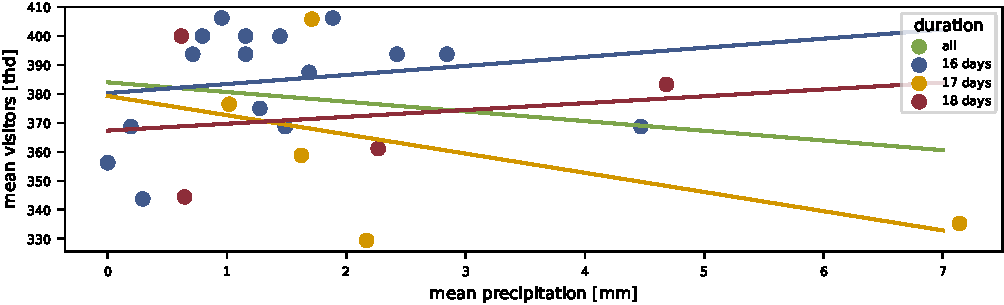
\includegraphics{fig/totalprecipitation.pdf}
  \caption{The mean daily visitors of the octoberfest as a function of the mean daily precipitation between 10am and 10pm at the time of the octoberfest in each year. The lines are the linear regression lines of the data points.}
  \label{figure_precipitation}
\end{figure*}\\
\noindent
In Figure~\ref{figure_precipitation} we can see the weak negative correlation in the green regression line which has a negative gradient while the values at both axis increas. The regression line shows that the mean daily amount of visitors of the octoberfest decrease by around 25.000 people as the mean precipitation at day time increases from zero milimeters to seven.\\


\section{Discussion \& Conclusion}\label{sec:conclusion}
The PCC is weak for the mean precipitation at day time and the mean daily vistors. This can have many reasons. One reason is, that we looked at the correlation of the mean over all days for each octoberfest and not at the correlation between the precipitation at each day and the visitor number of each day due to the lack of data. If in one year there is a very rainy day at which fewer people visit followed by good days with no rain were all the vistors come instead we couldn't see that the people that visited were influenced by the precipitation when only using the mean. Due to that even a weak correaltion shows that the amount of precipitation influences the amount of vistors. ........ In conclusion we can say, that the amount of precipitation influences the amount of visitors, but there are factors that influence the amount of precipitatioin more.\\

\section*{Contribution Statement}

Explain here, in one sentence per person, what each group member contributed. For example, you could write: Max Mustermann collected and prepared data. Gabi Musterfrau and John Doe performed the data analysis. Jane Doe produced visualizations. All authors will jointly wrote the text of the report. Note that you, as a group, a collectively responsible for the report. Your contributions should be roughly equal in amount and difficulty.

\section*{Notes} 

Your entire report has a \textbf{hard page limit of 4 pages} excluding references. (I.e. any pages beyond page 4 must only contain references). Appendices are \emph{not} possible. But you can put additional material, like interactive visualizations or videos, on a githunb repo (use \href{https://github.com/pnkraemer/tueplots}{links} in your pdf to refer to them). Each report has to contain \textbf{at least three plots or visualizations}, and \textbf{cite at least two references}. More details about how to prepare the report, inclucing how to produce plots, cite correctly, and how to ideally structure your github repo, will be discussed in the lecture, where a rubric for the evaluation will also be provided.


\bibliography{bibliography}
\bibliographystyle{icml2023}

\end{document}


% This document was modified from the file originally made available by
% Pat Langley and Andrea Danyluk for ICML-2K. This version was created
% by Iain Murray in 2018, and modified by Alexandre Bouchard in
% 2019 and 2021 and by Csaba Szepesvari, Gang Niu and Sivan Sabato in 2022.
% Modified again in 2023 by Sivan Sabato and Jonathan Scarlett.
% Previous contributors include Dan Roy, Lise Getoor and Tobias
% Scheffer, which was slightly modified from the 2010 version by
% Thorsten Joachims & Johannes Fuernkranz, slightly modified from the
% 2009 version by Kiri Wagstaff and Sam Roweis's 2008 version, which is
% slightly modified from Prasad Tadepalli's 2007 version which is a
% lightly changed version of the previous year's version by Andrew
% Moore, which was in turn edited from those of Kristian Kersting and
% Codrina Lauth. Alex Smola contributed to the algorithmic style files.
